\documentclass[ignorenonframetext,]{beamer}
\setbeamertemplate{caption}[numbered]
\setbeamertemplate{caption label separator}{: }
\setbeamercolor{caption name}{fg=normal text.fg}
\beamertemplatenavigationsymbolsempty
\usepackage{lmodern}
\usepackage{amssymb,amsmath}
\usepackage{ifxetex,ifluatex}
\usepackage{fixltx2e} % provides \textsubscript
\ifnum 0\ifxetex 1\fi\ifluatex 1\fi=0 % if pdftex
  \usepackage[T1]{fontenc}
  \usepackage[utf8]{inputenc}
\else % if luatex or xelatex
  \ifxetex
    \usepackage{mathspec}
  \else
    \usepackage{fontspec}
  \fi
  \defaultfontfeatures{Ligatures=TeX,Scale=MatchLowercase}
\fi
\usetheme[]{Madrid}
\usecolortheme{crane}
\usefonttheme{professionalfonts}
% use upquote if available, for straight quotes in verbatim environments
\IfFileExists{upquote.sty}{\usepackage{upquote}}{}
% use microtype if available
\IfFileExists{microtype.sty}{%
\usepackage{microtype}
\UseMicrotypeSet[protrusion]{basicmath} % disable protrusion for tt fonts
}{}
\newif\ifbibliography
\hypersetup{
            pdftitle={Introduction to R},
            pdfborder={0 0 0},
            breaklinks=true}
\urlstyle{same}  % don't use monospace font for urls
\usepackage{color}
\usepackage{fancyvrb}
\newcommand{\VerbBar}{|}
\newcommand{\VERB}{\Verb[commandchars=\\\{\}]}
\DefineVerbatimEnvironment{Highlighting}{Verbatim}{commandchars=\\\{\}}
% Add ',fontsize=\small' for more characters per line
\usepackage{framed}
\definecolor{shadecolor}{RGB}{248,248,248}
\newenvironment{Shaded}{\begin{snugshade}}{\end{snugshade}}
\newcommand{\KeywordTok}[1]{\textcolor[rgb]{0.13,0.29,0.53}{\textbf{#1}}}
\newcommand{\DataTypeTok}[1]{\textcolor[rgb]{0.13,0.29,0.53}{#1}}
\newcommand{\DecValTok}[1]{\textcolor[rgb]{0.00,0.00,0.81}{#1}}
\newcommand{\BaseNTok}[1]{\textcolor[rgb]{0.00,0.00,0.81}{#1}}
\newcommand{\FloatTok}[1]{\textcolor[rgb]{0.00,0.00,0.81}{#1}}
\newcommand{\ConstantTok}[1]{\textcolor[rgb]{0.00,0.00,0.00}{#1}}
\newcommand{\CharTok}[1]{\textcolor[rgb]{0.31,0.60,0.02}{#1}}
\newcommand{\SpecialCharTok}[1]{\textcolor[rgb]{0.00,0.00,0.00}{#1}}
\newcommand{\StringTok}[1]{\textcolor[rgb]{0.31,0.60,0.02}{#1}}
\newcommand{\VerbatimStringTok}[1]{\textcolor[rgb]{0.31,0.60,0.02}{#1}}
\newcommand{\SpecialStringTok}[1]{\textcolor[rgb]{0.31,0.60,0.02}{#1}}
\newcommand{\ImportTok}[1]{#1}
\newcommand{\CommentTok}[1]{\textcolor[rgb]{0.56,0.35,0.01}{\textit{#1}}}
\newcommand{\DocumentationTok}[1]{\textcolor[rgb]{0.56,0.35,0.01}{\textbf{\textit{#1}}}}
\newcommand{\AnnotationTok}[1]{\textcolor[rgb]{0.56,0.35,0.01}{\textbf{\textit{#1}}}}
\newcommand{\CommentVarTok}[1]{\textcolor[rgb]{0.56,0.35,0.01}{\textbf{\textit{#1}}}}
\newcommand{\OtherTok}[1]{\textcolor[rgb]{0.56,0.35,0.01}{#1}}
\newcommand{\FunctionTok}[1]{\textcolor[rgb]{0.00,0.00,0.00}{#1}}
\newcommand{\VariableTok}[1]{\textcolor[rgb]{0.00,0.00,0.00}{#1}}
\newcommand{\ControlFlowTok}[1]{\textcolor[rgb]{0.13,0.29,0.53}{\textbf{#1}}}
\newcommand{\OperatorTok}[1]{\textcolor[rgb]{0.81,0.36,0.00}{\textbf{#1}}}
\newcommand{\BuiltInTok}[1]{#1}
\newcommand{\ExtensionTok}[1]{#1}
\newcommand{\PreprocessorTok}[1]{\textcolor[rgb]{0.56,0.35,0.01}{\textit{#1}}}
\newcommand{\AttributeTok}[1]{\textcolor[rgb]{0.77,0.63,0.00}{#1}}
\newcommand{\RegionMarkerTok}[1]{#1}
\newcommand{\InformationTok}[1]{\textcolor[rgb]{0.56,0.35,0.01}{\textbf{\textit{#1}}}}
\newcommand{\WarningTok}[1]{\textcolor[rgb]{0.56,0.35,0.01}{\textbf{\textit{#1}}}}
\newcommand{\AlertTok}[1]{\textcolor[rgb]{0.94,0.16,0.16}{#1}}
\newcommand{\ErrorTok}[1]{\textcolor[rgb]{0.64,0.00,0.00}{\textbf{#1}}}
\newcommand{\NormalTok}[1]{#1}
\usepackage{graphicx,grffile}
\makeatletter
\def\maxwidth{\ifdim\Gin@nat@width>\linewidth\linewidth\else\Gin@nat@width\fi}
\def\maxheight{\ifdim\Gin@nat@height>\textheight0.8\textheight\else\Gin@nat@height\fi}
\makeatother
% Scale images if necessary, so that they will not overflow the page
% margins by default, and it is still possible to overwrite the defaults
% using explicit options in \includegraphics[width, height, ...]{}
\setkeys{Gin}{width=\maxwidth,height=\maxheight,keepaspectratio}

% Prevent slide breaks in the middle of a paragraph:
\widowpenalties 1 10000
\raggedbottom

\AtBeginPart{
  \let\insertpartnumber\relax
  \let\partname\relax
  \frame{\partpage}
}
\AtBeginSection{
  \ifbibliography
  \else
    \let\insertsectionnumber\relax
    \let\sectionname\relax
    \frame{\sectionpage}
  \fi
}
\AtBeginSubsection{
  \let\insertsubsectionnumber\relax
  \let\subsectionname\relax
  \frame{\subsectionpage}
}

\setlength{\parindent}{0pt}
\setlength{\parskip}{6pt plus 2pt minus 1pt}
\setlength{\emergencystretch}{3em}  % prevent overfull lines
\providecommand{\tightlist}{%
  \setlength{\itemsep}{0pt}\setlength{\parskip}{0pt}}
\setcounter{secnumdepth}{0}
\usepackage{booktabs}
\usepackage{hyperref}
\usepackage{caption}
\usepackage{graphicx}
\usepackage{amsmath}
\usepackage{graphics}
\author[SCC]{Statistical Consulting Centre}
\institute[\href{mailto:consulting@stat.auckland.ac.nz}
			{consulting@stat.auckland.ac.nz}]{\href{mailto:consulting@stat.auckland.ac.nz}
			{consulting@stat.auckland.ac.nz}\\
			The Department of Statistics\\
			The University of Auckland}
\titlegraphic{
\includegraphics[width=5cm]{..//..//S-DS-VC-RGB.png}}
\let\oldShaded\Shaded
\let\endoldShaded\endShaded
\renewenvironment{Shaded}{\footnotesize\oldShaded}{\endoldShaded}
\let\oldverbatim\verbatim
\let\endoldverbatim\endverbatim
\renewenvironment{verbatim}{\footnotesize\oldverbatim}{\endoldverbatim}

\title{Introduction to \textbf{R}}
\subtitle{Session 3 -- Basic R programming and data manipulation}
\date{9-10 July 2018}

\begin{document}
\frame{\titlepage}

\begin{frame}{Functions}

A function is a relationship between a set of inputs (arguments) and a
set of outputs. E.g., the function is fed some information on which it
operates, the results of which are the output.

\vspace{-30pt}

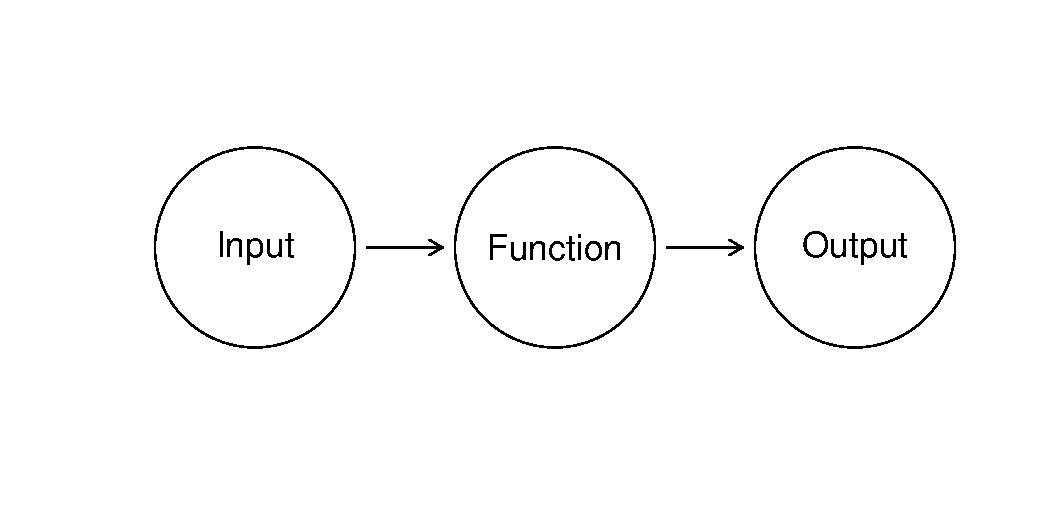
\includegraphics{Session3_files/figure-beamer/unnamed-chunk-1-1.pdf}
\vspace{-50pt}

This is an essential building block for the \textbf{R} package.

\end{frame}

\begin{frame}[fragile]{Functions}

We have seen many functions, e.g. \texttt{log()}, \texttt{mean()},
\texttt{table()}, \texttt{with()}, etc.

\vspace{-30pt}
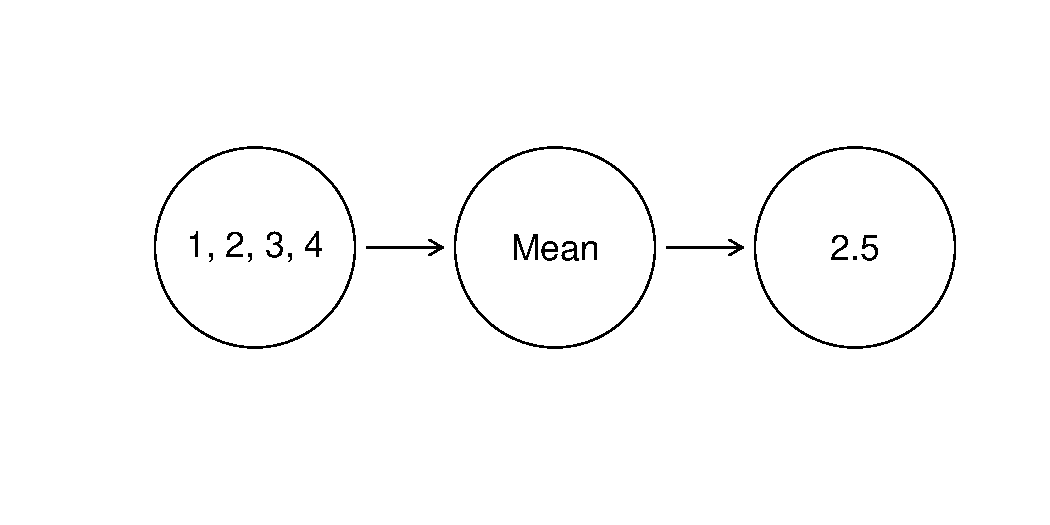
\includegraphics{Session3_files/figure-beamer/unnamed-chunk-2-1.pdf}

\end{frame}

\begin{frame}[fragile]{Working with functions}

\begin{itemize}
\tightlist
\item
  Functions can be user-defined, i.e., you can write your own.
\item
  \textbf{Output is the last line of the function.} You can use
  \texttt{return()} to specify the output.
\item
  Here is a function calculates the standard error of the mean (SEM):
  \vspace{-2pt} \[
  \mathrm{\hat{SEM}} = \frac{s}{\sqrt{N}}
  \] \vspace{-7pt}
\end{itemize}

\begin{Shaded}
\begin{Highlighting}[]
\NormalTok{mystder <-}\StringTok{ }\ControlFlowTok{function}\NormalTok{(x) \{}
\NormalTok{    mysd <-}\StringTok{ }\KeywordTok{sd}\NormalTok{(x, }\DataTypeTok{na.rm =} \OtherTok{TRUE}\NormalTok{)  }\CommentTok{# Calc std. deviation}
\NormalTok{    n <-}\StringTok{ }\KeywordTok{length}\NormalTok{(x)  }\CommentTok{# Calc sample size}
\NormalTok{    mysd}\OperatorTok{/}\KeywordTok{sqrt}\NormalTok{(n)  }\CommentTok{# Definition of SEM}
\NormalTok{\}}
\KeywordTok{mystder}\NormalTok{(patient.df}\OperatorTok{$}\NormalTok{Height)}
\end{Highlighting}
\end{Shaded}

\begin{verbatim}
## [1] 0.2586976
\end{verbatim}

\begin{itemize}
\tightlist
\item
  A set of user-defined functions can be bundled together into an
  \textbf{R} package.
\end{itemize}

\end{frame}

\begin{frame}[fragile]{\textbf{R} Packages}

\begin{itemize}
\item
  Currently, the CRAN package repository features 12,619 available
  packages (12 June 2018). There are about 15,310 CRAN, BioConductor and
  Github packages in total.
\item
  To install packages in \textbf{R}Studio, click on the
  \textbf{Packages} tab in the lower right, then:

  \begin{enumerate}
  \def\labelenumi{\arabic{enumi}.}
  \tightlist
  \item
    Click \texttt{Install}
  \item
    \texttt{Install\ from:\ Repository\ (CRAN)}
  \item
    Type the name of the package in \texttt{Packages}
  \item
    Click \textbf{Install}
  \end{enumerate}
\item
  Or, you can type \texttt{install.packages("}\emph{package
  name}\texttt{")}, e.g. \texttt{install.packages("plotrix")}.
\item
  After the installation, use \texttt{library("}\emph{package
  name}\texttt{")} to load it into \textbf{R}.
\end{itemize}

Note: Installation is performed only once; however, it must be loaded
(i.e.~use the command \texttt{install.packages("}\emph{package
name}\texttt{")} in \emph{every} \textbf{R} session.

\end{frame}

\begin{frame}[fragile]{Getting data into \textbf{R}}

\begin{itemize}
\tightlist
\item
  Base \textbf{R} includes only functions which read data sets saved in
  simple file formats, e.g. \texttt{csv}, \texttt{txt}, tab delimited,
  etc.
\item
  What if your data was saved in another format, e.g.~Excel?
\item
  The \texttt{readxl} package for \textbf{R} contains functions that may
  help, \url{https://cran.r-project.org/web/packages/readxl/index.html}
\end{itemize}

\begin{Shaded}
\begin{Highlighting}[]
\KeywordTok{library}\NormalTok{(readxl)}
\NormalTok{excel <-}\StringTok{ }\KeywordTok{read_excel}\NormalTok{(}\StringTok{"data.xlsx"}\NormalTok{, }\DataTypeTok{sheet =} \DecValTok{1}\NormalTok{)}
\end{Highlighting}
\end{Shaded}

\end{frame}

\begin{frame}[fragile]{Getting data into \textbf{R}}

\begin{itemize}
\tightlist
\item
  What if your data was saved in another format, e.g.~STATA, SPSS, or
  SAS?
\item
  The \texttt{haven} package for \textbf{R} contains functions that may
  help, \url{https://cran.r-project.org/web/packages/haven/index.html}
\end{itemize}

\begin{Shaded}
\begin{Highlighting}[]
\KeywordTok{library}\NormalTok{(haven)}
\NormalTok{stata <-}\StringTok{ }\KeywordTok{read_dta}\NormalTok{(}\StringTok{"data.dta"}\NormalTok{)}
\NormalTok{spss <-}\StringTok{ }\KeywordTok{read_sav}\NormalTok{(}\StringTok{"data.sav"}\NormalTok{)}
\NormalTok{sas <-}\StringTok{ }\KeywordTok{read_sas}\NormalTok{(}\StringTok{"data.sas7bdat"}\NormalTok{)}
\NormalTok{sasxport <-}\StringTok{ }\KeywordTok{read_xpt}\NormalTok{(}\StringTok{"data.xpt"}\NormalTok{)}
\end{Highlighting}
\end{Shaded}

However, it is always the easiest and safest to read data into
\textbf{R} from a \texttt{CSV} file.

\end{frame}

\begin{frame}[fragile]{Install \textbf{R} Packages from Bioconductor}

\begin{itemize}
\tightlist
\item
  To install core packages, type the following in an \textbf{R} Console
  panel:
\end{itemize}

\begin{Shaded}
\begin{Highlighting}[]
\KeywordTok{source}\NormalTok{(}\StringTok{"https://bioconductor.org/biocLite.R"}\NormalTok{)}
\KeywordTok{biocLite}\NormalTok{()}
\end{Highlighting}
\end{Shaded}

\vspace{-15pt}

\begin{itemize}
\item
  \texttt{source()} function reads \textbf{R} code from a file or, in
  this case, connection.
\item
  Install specific packages, e.g., \texttt{edgeR} and \texttt{limma},
  with
\end{itemize}

\begin{Shaded}
\begin{Highlighting}[]
\KeywordTok{source}\NormalTok{(}\StringTok{"https://bioconductor.org/biocLite.R"}\NormalTok{)}
\KeywordTok{biocLite}\NormalTok{(}\KeywordTok{c}\NormalTok{(}\StringTok{"edgeR"}\NormalTok{, }\StringTok{"limma"}\NormalTok{))}
\end{Highlighting}
\end{Shaded}

Note: Installation is performed only once; however, it must be loaded
(i.e.~use the command \texttt{install.packages("}\emph{package
name}\texttt{")} in \emph{every} \textbf{R} session.

\end{frame}

\begin{frame}[fragile]{Install \textbf{R} Packages from Github}

\begin{itemize}
\tightlist
\item
  To install \textbf{R} Packages from Github, you need to install
  \texttt{devtools} \textbf{R} package first, i.e.~type following in an
  \textbf{R} Console panel:
\end{itemize}

\begin{Shaded}
\begin{Highlighting}[]
\KeywordTok{install.packages}\NormalTok{(}\StringTok{"devtools"}\NormalTok{)}
\end{Highlighting}
\end{Shaded}

\begin{itemize}
\tightlist
\item
  Then, install specific packages from specific author's repositories,
  i.e.
\end{itemize}

\begin{Shaded}
\begin{Highlighting}[]
\NormalTok{devtools}\OperatorTok{::}\KeywordTok{install_github}\NormalTok{(}\StringTok{"author/package"}\NormalTok{)}
\end{Highlighting}
\end{Shaded}

\begin{itemize}
\tightlist
\item
  For example, with my \texttt{kcha193/infoDecompuTE} package, which
  exists at \url{https://github.com/kcha193/infoDecompuTE}, type the
  following in an \textbf{R} Console panel:
\end{itemize}

\begin{Shaded}
\begin{Highlighting}[]
\NormalTok{devtools}\OperatorTok{::}\KeywordTok{install_github}\NormalTok{(}\StringTok{"kcha193/infoDecompuTE"}\NormalTok{)}
\end{Highlighting}
\end{Shaded}

Note: Installation is performed only once; however, it must be loaded
(i.e.~use the command \texttt{install.packages("}\emph{package
name}\texttt{")} in \emph{every} \textbf{R} session.

\end{frame}

\begin{frame}[fragile]{Loading \textbf{R} Packages}

\begin{Shaded}
\begin{Highlighting}[]
\KeywordTok{library}\NormalTok{(dplyr)}
\end{Highlighting}
\end{Shaded}

\begin{verbatim}
## 
## Attaching package: 'dplyr'
\end{verbatim}

\begin{verbatim}
## The following objects are masked from 'package:stats':
## 
##     filter, lag
\end{verbatim}

\begin{verbatim}
## The following objects are masked from 'package:base':
## 
##     intersect, setdiff, setequal, union
\end{verbatim}

\vspace{-10pt}

\begin{itemize}
\tightlist
\item
  You can still use these functions from these packages by using two
  colons, e.g. \texttt{stats::filter()}.
\item
  Helps to access the exact function from that specific package.
\item
  this notation can be efficient if you only need to use a package's
  function once, e.g. \texttt{devtools::install\_github()}, as it avoids
  loading the package with \texttt{library()}.
\end{itemize}

\end{frame}

\begin{frame}[fragile]{Different types of data objects in \textbf{R}}

\textbf{R} has 6 different data types:

\begin{itemize}
\tightlist
\item
  character (alphanumeric; \texttt{"hello\ world"}), e.g. \texttt{Sex}
\item
  numeric (real or decimal; \texttt{3.14159}), e.g. \texttt{Patient.ID},
  \texttt{Age}, \texttt{Race}, \texttt{Weight}, \texttt{Height} and
  \texttt{Smoke}
\item
  integer (whole numbers; \texttt{256})
\item
  logical (\texttt{TRUE} or \texttt{FALSE}), e.g.
\end{itemize}

\begin{Shaded}
\begin{Highlighting}[]
\DecValTok{1} \OperatorTok{==}\StringTok{ }\DecValTok{1}
\end{Highlighting}
\end{Shaded}

\begin{verbatim}
## [1] TRUE
\end{verbatim}

\begin{Shaded}
\begin{Highlighting}[]
\DecValTok{2} \OperatorTok{<=}\StringTok{ }\DecValTok{0}
\end{Highlighting}
\end{Shaded}

\begin{verbatim}
## [1] FALSE
\end{verbatim}

\begin{Shaded}
\begin{Highlighting}[]
\DecValTok{3} \OperatorTok{!=}\StringTok{ }\DecValTok{2}
\end{Highlighting}
\end{Shaded}

\begin{verbatim}
## [1] TRUE
\end{verbatim}

\begin{itemize}
\tightlist
\item
  factor (numeric or alphanumeric, treated as categorical)
\item
  complex (numbers with imaginary components; \texttt{3i})
\end{itemize}

\end{frame}

\begin{frame}[fragile]{\texttt{factor}}

\begin{block}{What is a factor?}
    \textit{A variable which takes either qualitative values, ordinal values or a discrete set of quantitative values. The values of a factor are called its \emph{levels}.}
  \end{block}

Examples of factors:

\begin{itemize}
\tightlist
\item
  \texttt{Gender} with 2 \textbf{qualitative} levels: \texttt{Male} and
  \texttt{Female}.
\item
  \texttt{Education} with 6 \textbf{ordinal} levels: \texttt{None} \(<\)
  \texttt{Primary\ compl} \(<\) \texttt{Incpl\ secondary} \(<\)
  \texttt{Secondary\ compl} \(<\) \texttt{Incpl\ university} \(<\)
  \texttt{University\ degree}.
\item
  \texttt{Income} has 9 \textbf{quantitative} levels when the mid-values
  of the income ranges are used: \texttt{5000}, \texttt{12500},
  \texttt{17500}, \texttt{22500}, \texttt{27500}, \texttt{35000},
  \texttt{45000}, \texttt{60000} and \texttt{85000}.
\end{itemize}

\end{frame}

\begin{frame}{\texttt{factor}}

\begin{itemize}
\tightlist
\item
  \textbf{R} stores two \emph{additional} pieces of information for each
  factor: (1) the unique set of levels and (2) an integer value,
  assigned by \textbf{R}, for each unique level.
\item
  The integer values are assigned to factor levels so that they have an
  order associated with them.
\item
  By default, the unique levels are assigned the values 1, 2,\ldots{},
  according to ascending alphabetical order. This is not always
  appropriate!
\end{itemize}

\end{frame}

\begin{frame}[fragile]{\texttt{factor}}

\begin{Shaded}
\begin{Highlighting}[]
\KeywordTok{class}\NormalTok{(patient.df}\OperatorTok{$}\NormalTok{Sex)}
\end{Highlighting}
\end{Shaded}

\begin{verbatim}
## [1] "character"
\end{verbatim}

\begin{Shaded}
\begin{Highlighting}[]
\NormalTok{patient.df}\OperatorTok{$}\NormalTok{Sex <-}\StringTok{ }\KeywordTok{factor}\NormalTok{(patient.df}\OperatorTok{$}\NormalTok{Sex)}

\KeywordTok{class}\NormalTok{(patient.df}\OperatorTok{$}\NormalTok{Sex)}
\end{Highlighting}
\end{Shaded}

\begin{verbatim}
## [1] "factor"
\end{verbatim}

\begin{Shaded}
\begin{Highlighting}[]
\KeywordTok{levels}\NormalTok{(patient.df}\OperatorTok{$}\NormalTok{Sex)}
\end{Highlighting}
\end{Shaded}

\begin{verbatim}
## [1] "Female" "Male"
\end{verbatim}

\end{frame}

\begin{frame}[fragile]{\texttt{factor}}

\begin{Shaded}
\begin{Highlighting}[]
\NormalTok{patient.df}\OperatorTok{$}\NormalTok{BMI.group <-}\StringTok{ }\KeywordTok{factor}\NormalTok{(patient.df}\OperatorTok{$}\NormalTok{BMI.group)}
\KeywordTok{levels}\NormalTok{(patient.df}\OperatorTok{$}\NormalTok{BMI.group)}
\end{Highlighting}
\end{Shaded}

\begin{verbatim}
## [1] "normal"     "obese"      "overweight"
\end{verbatim}

\end{frame}

\begin{frame}[fragile]{\texttt{factor}}

\begin{Shaded}
\begin{Highlighting}[]
\NormalTok{patient.df}\OperatorTok{$}\NormalTok{BMI.group <-}\StringTok{ }\KeywordTok{factor}\NormalTok{(patient.df}\OperatorTok{$}\NormalTok{BMI.group, }
    \DataTypeTok{levels =} \KeywordTok{c}\NormalTok{(}\StringTok{"normal"}\NormalTok{, }\StringTok{"overweight"}\NormalTok{, }\StringTok{"obese"}\NormalTok{))}
\KeywordTok{levels}\NormalTok{(patient.df}\OperatorTok{$}\NormalTok{BMI.group)}
\end{Highlighting}
\end{Shaded}

\begin{verbatim}
## [1] "normal"     "overweight" "obese"
\end{verbatim}

\end{frame}

\begin{frame}[fragile]{Which other variables should also be
\texttt{factors}?}

\begin{Shaded}
\begin{Highlighting}[]
\KeywordTok{str}\NormalTok{(patient.df)}
\end{Highlighting}
\end{Shaded}

\begin{verbatim}
## 'data.frame':    200 obs. of  9 variables:
##  $ Patient.ID : int  3 4 9 10 11 19 34 44 45 48 ...
##  $ Age        : int  21 32 48 35 48 44 42 24 67 56 ...
##  $ Sex        : Factor w/ 2 levels "Female","Male": 2 1 1 2 2 2 1 1 1 1 ...
##  $ Weight     : num  180 NA 150 204 155 ...
##  $ Height     : num  70.4 63.9 61.8 69.8 NA 70.2 62.6 64.4 64.3 67.6 ...
##  $ Smoke.group: chr  NA NA "No" NA ...
##  $ Race.group : chr  "Caucasian" "Caucasian" "Caucasian" "Caucasian" ...
##  $ BMI        : num  25.5 NA 27.6 29.4 NA ...
##  $ BMI.group  : Factor w/ 3 levels "normal","overweight",..: 2 NA 2 2 NA 2 1 1 2 3 ...
\end{verbatim}

\end{frame}

\begin{frame}[fragile]{Which other variables should also be
\texttt{factors}?}

\begin{Shaded}
\begin{Highlighting}[]
\NormalTok{patient.df}\OperatorTok{$}\NormalTok{Race.group <-}\StringTok{ }\KeywordTok{factor}\NormalTok{(patient.df}\OperatorTok{$}\NormalTok{Race.group)}
\NormalTok{patient.df}\OperatorTok{$}\NormalTok{Smoke.group <-}\StringTok{ }\KeywordTok{factor}\NormalTok{(patient.df}\OperatorTok{$}\NormalTok{Smoke.group)}
\end{Highlighting}
\end{Shaded}

\end{frame}

\begin{frame}[fragile]{Converting numbers to \texttt{factors}}

\begin{Shaded}
\begin{Highlighting}[]
\NormalTok{test <-}\StringTok{ }\KeywordTok{factor}\NormalTok{(}\KeywordTok{c}\NormalTok{(}\DecValTok{0}\NormalTok{, }\DecValTok{1}\NormalTok{, }\DecValTok{2}\NormalTok{))}
\NormalTok{test}
\end{Highlighting}
\end{Shaded}

\begin{verbatim}
## [1] 0 1 2
## Levels: 0 1 2
\end{verbatim}

\begin{itemize}
\tightlist
\item
  then convert back to numbers?
\end{itemize}

\end{frame}

\begin{frame}[fragile]{And convert \texttt{factor} back to numbers}

\begin{itemize}
\tightlist
\item
  Need to convert it to character first, using \texttt{as.character()},
  then convert back to numbers, using \texttt{as.numeric()}.
\end{itemize}

\begin{Shaded}
\begin{Highlighting}[]
\NormalTok{test}
\end{Highlighting}
\end{Shaded}

\begin{verbatim}
## [1] 0 1 2
## Levels: 0 1 2
\end{verbatim}

\begin{Shaded}
\begin{Highlighting}[]
\KeywordTok{as.numeric}\NormalTok{(test)}
\end{Highlighting}
\end{Shaded}

\begin{verbatim}
## [1] 1 2 3
\end{verbatim}

\begin{Shaded}
\begin{Highlighting}[]
\KeywordTok{as.numeric}\NormalTok{(}\KeywordTok{as.character}\NormalTok{(test))}
\end{Highlighting}
\end{Shaded}

\begin{verbatim}
## [1] 0 1 2
\end{verbatim}

\end{frame}

\begin{frame}[fragile]{Your turn (Binning ages into age groups)}

\begin{itemize}
\tightlist
\item
  Sometimes we are interested in examining responses by age group.
\item
  Now, assign each of the 200 patients to one of three age groups:
  ``Under 35'', ``36 to 60'' and ``Over 61''.
\item
  Convert \texttt{Age.group} to a \texttt{factor} with levels in
  ascending order.
\end{itemize}

\end{frame}

\begin{frame}[fragile]{Your turn (Binning ages into age groups)}

Assign each of the 200 patients to one of three age groups: ``Under
35'', ``36 to 60'' and ``Over 61''.

\begin{Shaded}
\begin{Highlighting}[]
\NormalTok{patient.df}\OperatorTok{$}\NormalTok{Age.group <-}\StringTok{ }
\StringTok{  }\KeywordTok{ifelse}\NormalTok{(patient.df}\OperatorTok{$}\NormalTok{Age}\OperatorTok{<=}\DecValTok{35}\NormalTok{, }\StringTok{"Under 35"}\NormalTok{, }
         \KeywordTok{ifelse}\NormalTok{(patient.df}\OperatorTok{$}\NormalTok{Age }\OperatorTok{<=}\StringTok{ }\DecValTok{60}\NormalTok{, }\StringTok{"36 to 60"}\NormalTok{, }\StringTok{"Over 61"}\NormalTok{))}
\KeywordTok{table}\NormalTok{(patient.df}\OperatorTok{$}\NormalTok{Age.group)}
\end{Highlighting}
\end{Shaded}

\begin{verbatim}
## 
## 36 to 60  Over 61 Under 35 
##       65       68       67
\end{verbatim}

\end{frame}

\begin{frame}[fragile]{Your turn (Binning ages into age groups)}

Convert \texttt{Age.group} to a \texttt{factor} with levels in ascending
order.

\begin{Shaded}
\begin{Highlighting}[]
\NormalTok{patient.df}\OperatorTok{$}\NormalTok{Age.group <-}\StringTok{ }\KeywordTok{factor}\NormalTok{(patient.df}\OperatorTok{$}\NormalTok{Age.group)}
\KeywordTok{table}\NormalTok{(patient.df}\OperatorTok{$}\NormalTok{Age.group)}
\end{Highlighting}
\end{Shaded}

\begin{verbatim}
## 
## 36 to 60  Over 61 Under 35 
##       65       68       67
\end{verbatim}

\end{frame}

\begin{frame}[fragile]{Your turn (Binning ages into age groups)}

Convert \texttt{Age.group} to a \texttt{factor} with levels in ascending
order.

\begin{Shaded}
\begin{Highlighting}[]
\NormalTok{patient.df}\OperatorTok{$}\NormalTok{Age.group <-}\StringTok{ }\KeywordTok{factor}\NormalTok{(patient.df}\OperatorTok{$}\NormalTok{Age.group, }
    \DataTypeTok{levels =} \KeywordTok{c}\NormalTok{(}\StringTok{"Under 35"}\NormalTok{, }\StringTok{"36 to 60"}\NormalTok{, }\StringTok{"Over 61"}\NormalTok{))}
\KeywordTok{table}\NormalTok{(patient.df}\OperatorTok{$}\NormalTok{Age.group)}
\end{Highlighting}
\end{Shaded}

\begin{verbatim}
## 
## Under 35 36 to 60  Over 61 
##       67       65       68
\end{verbatim}

\end{frame}

\begin{frame}[fragile]{Other way: \texttt{if}/\texttt{else} statement}

\begin{Shaded}
\begin{Highlighting}[]
\ControlFlowTok{if}\NormalTok{ (test) \{}
    \CommentTok{# yes}
\NormalTok{\} }\ControlFlowTok{else}\NormalTok{ \{}
    \CommentTok{# no}
\NormalTok{\}}
\end{Highlighting}
\end{Shaded}

\begin{itemize}
\tightlist
\item
  \texttt{test}: a logical test.
\item
  \texttt{yes}, what happens if the test is True.
\item
  \texttt{no}, what happens if the test is False.
\end{itemize}

\end{frame}

\begin{frame}[fragile]{Other way: \texttt{if}/\texttt{else} statement}

\begin{Shaded}
\begin{Highlighting}[]
\ControlFlowTok{if}\NormalTok{ (test) \{}
    \CommentTok{# yes for (test)}
\NormalTok{\} }\ControlFlowTok{else} \ControlFlowTok{if}\NormalTok{ (test1) \{}
    \CommentTok{# no for (test) but yes for (test1)}
\NormalTok{\} }\ControlFlowTok{else}\NormalTok{ \{}
    \CommentTok{# no for both (test) and (test1)}
\NormalTok{\}}
\end{Highlighting}
\end{Shaded}

\end{frame}

\begin{frame}{Relational data}

\begin{itemize}
\item
  In general, it is rare in data analysis involves only a single table
  of data.
\item
  Examples:

  \begin{itemize}
  \tightlist
  \item
    Patient information and blood test measurements
  \item
    Experimental design and measurements from the high-throughput
    biological instrument
  \end{itemize}
\end{itemize}

\end{frame}

\begin{frame}[fragile]{\texttt{cholesterol.df}}

Serum Cholesterol level, mg/100ml, measured on:

\begin{itemize}
\tightlist
\item
  \texttt{Day1}
\item
  \texttt{Day5}
\item
  \texttt{Day10}
\end{itemize}

\end{frame}

\begin{frame}[fragile]{Reading data into \textbf{R}}

\begin{Shaded}
\begin{Highlighting}[]
\KeywordTok{setwd}\NormalTok{(}\StringTok{"your working directory"}\NormalTok{)}
\NormalTok{cholesterol.df <-}\StringTok{ }\KeywordTok{read.csv}\NormalTok{(}\StringTok{"Data/CholesterolNA.csv"}\NormalTok{)}
\KeywordTok{head}\NormalTok{(cholesterol.df)}
\end{Highlighting}
\end{Shaded}

\begin{verbatim}
##   Patient.ID Day1 Day5 Day10
## 1          3  268  276   281
## 2          4  160  170   170
## 3          9  236  245   252
## 4         10  225  231   235
## 5         11  260  256   257
## 6         19  187  194   195
\end{verbatim}

\end{frame}

\begin{frame}[fragile]{\texttt{names()}, \texttt{dim()} and
\texttt{str()} functions}

\begin{Shaded}
\begin{Highlighting}[]
\KeywordTok{names}\NormalTok{(cholesterol.df)}
\end{Highlighting}
\end{Shaded}

\begin{verbatim}
## [1] "Patient.ID" "Day1"       "Day5"      
## [4] "Day10"
\end{verbatim}

\begin{Shaded}
\begin{Highlighting}[]
\KeywordTok{dim}\NormalTok{(cholesterol.df)}
\end{Highlighting}
\end{Shaded}

\begin{verbatim}
## [1] 200   4
\end{verbatim}

\begin{Shaded}
\begin{Highlighting}[]
\KeywordTok{str}\NormalTok{(cholesterol.df)}
\end{Highlighting}
\end{Shaded}

\begin{verbatim}
## 'data.frame':    200 obs. of  4 variables:
##  $ Patient.ID: int  3 4 9 10 11 19 34 44 45 48 ...
##  $ Day1      : int  268 160 236 225 260 187 216 137 NA 156 ...
##  $ Day5      : int  276 170 245 231 256 194 212 135 NA 157 ...
##  $ Day10     : int  281 170 252 235 257 195 222 136 NA 159 ...
\end{verbatim}

\end{frame}

\begin{frame}[fragile]{Combining data frame by columns
(\texttt{cbind()})}

\begin{Shaded}
\begin{Highlighting}[]
\NormalTok{combined.df <-}\StringTok{ }\KeywordTok{cbind}\NormalTok{(patient.df, cholesterol.df[, }\OperatorTok{-}\DecValTok{1}\NormalTok{])}
\end{Highlighting}
\end{Shaded}

\begin{itemize}
\tightlist
\item
  Thus, the function for combining the data-frame by rows is
  \texttt{rbind()}.
\item
  Make sure the dimensions are correct for two combining data-frames.
\item
  Also, you need to make sure each row in \texttt{patient.df} matches
  each row in \texttt{cholesterol.df}.
\end{itemize}

\end{frame}

\begin{frame}[fragile]{Reading data into \textbf{R} (Again)}

\begin{Shaded}
\begin{Highlighting}[]
\KeywordTok{setwd}\NormalTok{(}\StringTok{"your working directory"}\NormalTok{)}
\NormalTok{cholesterol.df <-}\StringTok{ }\KeywordTok{read.csv}\NormalTok{(}\StringTok{"Data/Cholesterol.csv"}\NormalTok{)}
\KeywordTok{head}\NormalTok{(cholesterol.df)}
\end{Highlighting}
\end{Shaded}

\begin{verbatim}
##   Patient.ID Day1 Day5 Day10
## 1          3  268  276   281
## 2          4  160  170   170
## 3          9  236  245   252
## 4         10  225  231   235
## 5         11  260  256   257
## 6         19  187  194   195
\end{verbatim}

\end{frame}

\begin{frame}[fragile]{\texttt{names()}, \texttt{dim()} and
\texttt{str()} functions}

\begin{Shaded}
\begin{Highlighting}[]
\CommentTok{# Names of the variables}
\KeywordTok{names}\NormalTok{(cholesterol.df)}
\end{Highlighting}
\end{Shaded}

\begin{verbatim}
## [1] "Patient.ID" "Day1"       "Day5"      
## [4] "Day10"
\end{verbatim}

\begin{Shaded}
\begin{Highlighting}[]
\KeywordTok{dim}\NormalTok{(cholesterol.df)}
\end{Highlighting}
\end{Shaded}

\begin{verbatim}
## [1] 186   4
\end{verbatim}

\begin{Shaded}
\begin{Highlighting}[]
\KeywordTok{str}\NormalTok{(cholesterol.df)}
\end{Highlighting}
\end{Shaded}

\begin{verbatim}
## 'data.frame':    186 obs. of  4 variables:
##  $ Patient.ID: int  3 4 9 10 11 19 34 44 48 49 ...
##  $ Day1      : int  268 160 236 225 260 187 216 137 156 179 ...
##  $ Day5      : int  276 170 245 231 256 194 212 135 157 183 ...
##  $ Day10     : int  281 170 252 235 257 195 222 136 159 183 ...
\end{verbatim}

\end{frame}

\begin{frame}[fragile]{Combining data frame by columns
(\texttt{cbind()})}

\begin{Shaded}
\begin{Highlighting}[]
\NormalTok{combined.df <-}\StringTok{ }\KeywordTok{cbind}\NormalTok{(patient.df, cholesterol.df)}
\end{Highlighting}
\end{Shaded}

\begin{verbatim}
## Error in data.frame(..., check.names = FALSE): arguments imply differing number of rows: 200, 186
\end{verbatim}

\end{frame}

\begin{frame}[fragile]{Solution}

\begin{itemize}
\tightlist
\item
  Combining the based on the \texttt{Patient.ID} in both
  \texttt{patient.df} and \texttt{cholesterol.df}.
\item
  First thing is to make sure the \texttt{Patient.ID} are unique in both
  data-frames.
\end{itemize}

\end{frame}

\begin{frame}[fragile]{Solution}

\begin{itemize}
\tightlist
\item
  Combining the based on the \texttt{Patient.ID} in both
  \texttt{patient.df} and \texttt{cholesterol.df}.
\item
  First thing is to make sure the \texttt{Patient.ID} are unique in both
  data-frames.
\end{itemize}

\begin{Shaded}
\begin{Highlighting}[]
\KeywordTok{sum}\NormalTok{(}\KeywordTok{table}\NormalTok{(patient.df}\OperatorTok{$}\NormalTok{Patient.ID) }\OperatorTok{>}\StringTok{ }\DecValTok{1}\NormalTok{)}
\end{Highlighting}
\end{Shaded}

\begin{verbatim}
## [1] 0
\end{verbatim}

\begin{Shaded}
\begin{Highlighting}[]
\KeywordTok{sum}\NormalTok{(}\KeywordTok{table}\NormalTok{(cholesterol.df}\OperatorTok{$}\NormalTok{Patient.ID) }\OperatorTok{>}\StringTok{ }\DecValTok{1}\NormalTok{)}
\end{Highlighting}
\end{Shaded}

\begin{verbatim}
## [1] 0
\end{verbatim}

\end{frame}

\begin{frame}[fragile]{\texttt{dplyr} \textbf{R} package}

\begin{itemize}
\tightlist
\item
  \texttt{dplyr} \textbf{R} package provides some useful functions that
  correspond to the most data manipulation tasks.
\end{itemize}

\begin{Shaded}
\begin{Highlighting}[]
\KeywordTok{library}\NormalTok{(dplyr)}
\end{Highlighting}
\end{Shaded}

\begin{itemize}
\tightlist
\item
  Mutating joins allow you to combine variables from multiple tables,
  there are four common types:

  \begin{itemize}
  \tightlist
  \item
    \texttt{left\_join()}
  \item
    \texttt{right\_join()}
  \item
    \texttt{full\_join()}
  \item
    \texttt{inner\_join()}
  \end{itemize}
\end{itemize}

\end{frame}

\begin{frame}[fragile]{\texttt{dplyr} \textbf{R} package}

\begin{Shaded}
\begin{Highlighting}[]
\NormalTok{x <-}\StringTok{ }\KeywordTok{data.frame}\NormalTok{(}\DataTypeTok{key =} \KeywordTok{c}\NormalTok{(}\DecValTok{1}\NormalTok{,}\DecValTok{2}\NormalTok{,}\DecValTok{3}\NormalTok{), }\DataTypeTok{val.x =} \KeywordTok{c}\NormalTok{(}\StringTok{"x1"}\NormalTok{,}\StringTok{"x2"}\NormalTok{,}\StringTok{"x3"}\NormalTok{))}
\NormalTok{y <-}\StringTok{ }\KeywordTok{data.frame}\NormalTok{(}\DataTypeTok{key =} \KeywordTok{c}\NormalTok{(}\DecValTok{1}\NormalTok{,}\DecValTok{2}\NormalTok{,}\DecValTok{4}\NormalTok{), }\DataTypeTok{val.y =} \KeywordTok{c}\NormalTok{(}\StringTok{"y1"}\NormalTok{,}\StringTok{"y2"}\NormalTok{,}\StringTok{"y4"}\NormalTok{))}
\end{Highlighting}
\end{Shaded}

\begin{table}[!htb]
    \begin{minipage}{.5\linewidth}
      \caption*{Data-frame x}
      \centering 
\begin{tabular}{rl}
\toprule
key & val.x\\
\midrule
1 & x1\\
2 & x2\\
3 & x3\\
\bottomrule
\end{tabular} \end{minipage}%
    \begin{minipage}{.5\linewidth}
      \centering
        \caption*{Data-frame y} 
\begin{tabular}{rl}
\toprule
key & val.y\\
\midrule
1 & y1\\
2 & y2\\
4 & y4\\
\bottomrule
\end{tabular} \end{minipage} 
\end{table}

\end{frame}

\begin{frame}[fragile]{\texttt{left\_join()}}

\begin{Shaded}
\begin{Highlighting}[]
\KeywordTok{left_join}\NormalTok{(x, y, }\DataTypeTok{by =} \StringTok{"key"}\NormalTok{)}
\end{Highlighting}
\end{Shaded}

\begin{itemize}
\tightlist
\item
  return all rows from \texttt{x}, and all columns from \texttt{x} and
  \texttt{y}.
\item
  Rows in \texttt{x} with no match in y will have \texttt{NA} values in
  the new columns.
\item
  If there are multiple matches between \texttt{x} and \texttt{y}, all
  combinations of the matches are returned.
\end{itemize}

\begin{table}[!htb]
    \begin{minipage}{.33\linewidth}
      \caption*{Data-frame x}
      \centering 
\begin{tabular}{rl}
\toprule
key & val.x\\
\midrule
1 & x1\\
2 & x2\\
3 & x3\\
\bottomrule
\end{tabular} \end{minipage}%
    \begin{minipage}{.33\linewidth}
      \centering
        \caption*{Data-frame y} 
\begin{tabular}{rl}
\toprule
key & val.y\\
\midrule
1 & y1\\
2 & y2\\
4 & y4\\
\bottomrule
\end{tabular} \end{minipage}%
    \begin{minipage}{.33\linewidth}
      \centering
        \caption*{left join} 
\begin{tabular}{rll}
\toprule
key & val.x & val.y\\
\midrule
1 & x1 & y1\\
2 & x2 & y2\\
3 & x3 & NA\\
\bottomrule
\end{tabular} \end{minipage} 
\end{table}

\end{frame}

\begin{frame}[fragile]{\texttt{right\_join()}}

\begin{Shaded}
\begin{Highlighting}[]
\KeywordTok{right_join}\NormalTok{(x, y, }\DataTypeTok{by =} \StringTok{"key"}\NormalTok{)}
\end{Highlighting}
\end{Shaded}

\begin{itemize}
\tightlist
\item
  return all rows from \texttt{y}, and all columns from \texttt{x} and
  \texttt{y}.
\item
  Rows in \texttt{y} with no match in x will have \texttt{NA} values in
  the new columns.
\item
  If there are multiple matches between \texttt{x} and \texttt{y}, all
  combinations of the matches are returned.
\end{itemize}

\begin{table}[!htb]
    \begin{minipage}{.33\linewidth}
      \caption*{Data-frame x}
      \centering 
\begin{tabular}{rl}
\toprule
key & val.x\\
\midrule
1 & x1\\
2 & x2\\
3 & x3\\
\bottomrule
\end{tabular} \end{minipage}%
    \begin{minipage}{.33\linewidth}
      \centering
        \caption*{Data-frame y} 
\begin{tabular}{rl}
\toprule
key & val.y\\
\midrule
1 & y1\\
2 & y2\\
4 & y4\\
\bottomrule
\end{tabular} \end{minipage}%
    \begin{minipage}{.33\linewidth}
      \centering
        \caption*{right join} 
\begin{tabular}{rll}
\toprule
key & val.x & val.y\\
\midrule
1 & x1 & y1\\
2 & x2 & y2\\
4 & NA & y4\\
\bottomrule
\end{tabular} \end{minipage} 
\end{table}

\end{frame}

\begin{frame}[fragile]{\texttt{full\_join()}}

\begin{Shaded}
\begin{Highlighting}[]
\KeywordTok{full_join}\NormalTok{(x, y, }\DataTypeTok{by =} \StringTok{"key"}\NormalTok{)}
\end{Highlighting}
\end{Shaded}

\begin{itemize}
\tightlist
\item
  return all rows and all columns from both \texttt{x} and \texttt{y}.
\item
  Where there are not matching values, returns \texttt{NA} for the one
  missing.
\end{itemize}

\begin{table}[!htb]
    \begin{minipage}{.33\linewidth}
      \caption*{Data-frame x}
      \centering 
\begin{tabular}{rl}
\toprule
key & val.x\\
\midrule
1 & x1\\
2 & x2\\
3 & x3\\
\bottomrule
\end{tabular} \end{minipage}%
    \begin{minipage}{.33\linewidth}
      \centering
        \caption*{Data-frame y} 
\begin{tabular}{rl}
\toprule
key & val.y\\
\midrule
1 & y1\\
2 & y2\\
4 & y4\\
\bottomrule
\end{tabular} \end{minipage}%
    \begin{minipage}{.33\linewidth}
      \centering
        \caption*{full join} 
\begin{tabular}{rll}
\toprule
key & val.x & val.y\\
\midrule
1 & x1 & y1\\
2 & x2 & y2\\
3 & x3 & NA\\
4 & NA & y4\\
\bottomrule
\end{tabular} \end{minipage} 
\end{table}

\end{frame}

\begin{frame}[fragile]{\texttt{inner\_join()}}

\begin{Shaded}
\begin{Highlighting}[]
\KeywordTok{inner_join}\NormalTok{(x, y, }\DataTypeTok{by =} \StringTok{"key"}\NormalTok{)}
\end{Highlighting}
\end{Shaded}

\begin{itemize}
\tightlist
\item
  return all rows from \texttt{x} where there are matching values in
  \texttt{y}, and all columns from \texttt{x} and \texttt{y}.
\item
  If there are multiple matches between \texttt{x} and \texttt{y}, all
  combination of the matches are returned.
\end{itemize}

\begin{table}[!htb]
    \begin{minipage}{.33\linewidth}
      \caption*{Data-frame x}
      \centering 
\begin{tabular}{rl}
\toprule
key & val.x\\
\midrule
1 & x1\\
2 & x2\\
3 & x3\\
\bottomrule
\end{tabular} \end{minipage}%
    \begin{minipage}{.33\linewidth}
      \centering
        \caption*{Data-frame y} 
\begin{tabular}{rl}
\toprule
key & val.y\\
\midrule
1 & y1\\
2 & y2\\
4 & y4\\
\bottomrule
\end{tabular} \end{minipage}%
    \begin{minipage}{.33\linewidth}
      \centering
        \caption*{inner join} 
\begin{tabular}{rll}
\toprule
key & val.x & val.y\\
\midrule
1 & x1 & y1\\
2 & x2 & y2\\
\bottomrule
\end{tabular} \end{minipage} 
\end{table}

\end{frame}

\begin{frame}[fragile]{\texttt{dplyr} \textbf{R} package}

These four types of mutating join are differ in their behavior when a
match is not found.

\begin{itemize}
\tightlist
\item
  \texttt{left\_join()}
\item
  \texttt{right\_join()}
\item
  \texttt{full\_join()}
\item
  \texttt{inner\_join()}
\end{itemize}

Which one should we use for \texttt{patient.df} and
\texttt{cholesterol.df} data-frames?

\end{frame}

\begin{frame}[fragile]{Combining two data frames}

\begin{Shaded}
\begin{Highlighting}[]
\NormalTok{combined.df <-}\StringTok{ }\KeywordTok{left_join}\NormalTok{(patient.df, cholesterol.df)}
\end{Highlighting}
\end{Shaded}

\begin{verbatim}
## Joining, by = "Patient.ID"
\end{verbatim}

\begin{Shaded}
\begin{Highlighting}[]
\NormalTok{combined.df <-}\StringTok{ }\KeywordTok{left_join}\NormalTok{(patient.df, cholesterol.df, }
    \DataTypeTok{by =} \StringTok{"Patient.ID"}\NormalTok{)}
\end{Highlighting}
\end{Shaded}

\begin{itemize}
\tightlist
\item
  Variable names:
\end{itemize}

\begin{Shaded}
\begin{Highlighting}[]
\KeywordTok{names}\NormalTok{(combined.df)}
\end{Highlighting}
\end{Shaded}

\begin{verbatim}
##  [1] "Patient.ID"  "Age"         "Sex"        
##  [4] "Weight"      "Height"      "Smoke.group"
##  [7] "Race.group"  "BMI"         "BMI.group"  
## [10] "Age.group"   "Day1"        "Day5"       
## [13] "Day10"
\end{verbatim}

\end{frame}

\begin{frame}[fragile]{Combining two data frames}

\begin{Shaded}
\begin{Highlighting}[]
\KeywordTok{str}\NormalTok{(combined.df)}
\end{Highlighting}
\end{Shaded}

\begin{verbatim}
## 'data.frame':    200 obs. of  13 variables:
##  $ Patient.ID : int  3 4 9 10 11 19 34 44 45 48 ...
##  $ Age        : int  21 32 48 35 48 44 42 24 67 56 ...
##  $ Sex        : Factor w/ 2 levels "Female","Male": 2 1 1 2 2 2 1 1 1 1 ...
##  $ Weight     : num  180 NA 150 204 155 ...
##  $ Height     : num  70.4 63.9 61.8 69.8 NA 70.2 62.6 64.4 64.3 67.6 ...
##  $ Smoke.group: Factor w/ 2 levels "No","Yes": NA NA 1 NA 1 2 2 2 NA 1 ...
##  $ Race.group : Factor w/ 3 levels "African","Caucasian",..: 2 2 2 2 2 1 1 2 1 2 ...
##  $ BMI        : num  25.5 NA 27.6 29.4 NA ...
##  $ BMI.group  : Factor w/ 3 levels "normal","overweight",..: 2 NA 2 2 NA 2 1 1 2 3 ...
##  $ Age.group  : Factor w/ 3 levels "Under 35","36 to 60",..: 1 1 2 1 2 2 2 1 3 2 ...
##  $ Day1       : int  268 160 236 225 260 187 216 137 NA 156 ...
##  $ Day5       : int  276 170 245 231 256 194 212 135 NA 157 ...
##  $ Day10      : int  281 170 252 235 257 195 222 136 NA 159 ...
\end{verbatim}

\end{frame}

\begin{frame}[fragile]{Renaming variables}

You can change the variable names.

\begin{Shaded}
\begin{Highlighting}[]
\KeywordTok{names}\NormalTok{(combined.df)[}\KeywordTok{c}\NormalTok{(}\DecValTok{1}\NormalTok{,}\DecValTok{11}\NormalTok{,}\DecValTok{12}\NormalTok{,}\DecValTok{13}\NormalTok{)] <-}\StringTok{ }
\StringTok{  }\KeywordTok{c}\NormalTok{(}\StringTok{"ID"}\NormalTok{, }\StringTok{"Baseline"}\NormalTok{, }\StringTok{"PreTrt"}\NormalTok{, }\StringTok{"PostTrt"}\NormalTok{)}

\KeywordTok{names}\NormalTok{(combined.df)}
\end{Highlighting}
\end{Shaded}

\begin{verbatim}
##  [1] "ID"          "Age"         "Sex"        
##  [4] "Weight"      "Height"      "Smoke.group"
##  [7] "Race.group"  "BMI"         "BMI.group"  
## [10] "Age.group"   "Baseline"    "PreTrt"     
## [13] "PostTrt"
\end{verbatim}

\end{frame}

\begin{frame}[fragile]{Summary}

\begin{itemize}
\tightlist
\item
  functions
\item
  \textbf{R} packages
\item
  \texttt{factor}
\item
  Combining two data frames
\end{itemize}

\end{frame}

\end{document}
